%%%%%%%%%%%%%%%%%%%%%%%%%%%%%%%%%%%%%%%%%
%  My documentation report
%  Objetive: Explain what I did and how, so someone can continue with the investigation
%
% Important note:
% Chapter heading images should have a 2:1 width:height ratio,
% e.g. 920px width and 460px height.
%
%%%%%%%%%%%%%%%%%%%%%%%%%%%%%%%%%%%%%%%%%


%----------------------------------------------------------------------------------------
%	PACKAGES AND OTHER DOCUMENT CONFIGURATIONS
%----------------------------------------------------------------------------------------

\documentclass[11pt,fleqn]{book} % Default font size and left-justified equations

\usepackage[top=3cm,bottom=3cm,left=3.2cm,right=3.2cm,headsep=10pt,letterpaper]{geometry} % Page margins

\usepackage{xcolor} % Required for specifying colors by name
\definecolor{ocre}{RGB}{52,177,201} % Define the orange color used for highlighting throughout the book

% Font Settings
\usepackage{avant} % Use the Avantgarde font for headings
%\usepackage{times} % Use the Times font for headings
\usepackage{mathptmx} % Use the Adobe Times Roman as the default text font together with math symbols from the Sym­bol, Chancery and Com­puter Modern fonts
\usepackage{microtype} % Slightly tweak font spacing for aesthetics
\usepackage[utf8]{inputenc} % Required for including letters with accents
\usepackage[T1]{fontenc} % Use 8-bit encoding that has 256 glyphs
\usepackage{amsthm}

% Bibliography
\usepackage{csquotes}
\usepackage[style=alphabetic,sorting=nyt,sortcites=true,autopunct=true,autolang=hyphen,hyperref=true,abbreviate=false,backref=true,backend=biber]{biblatex}
\addbibresource{bibliography.bib} % BibTeX bibliography file
\defbibheading{bibempty}{}

%----------------------------------------------------------------------------------------
%	VARIOUS REQUIRED PACKAGES
%----------------------------------------------------------------------------------------

\usepackage{titlesec} % Allows customization of titles

\usepackage{graphicx} % Required for including pictures
\graphicspath{{Pictures/}} % Specifies the directory where pictures are stored
% \graphicspath{{Plots/}}
\usepackage{lipsum} % Inserts dummy text

\usepackage{tikz} % Required for drawing custom shapes

\usepackage[english]{babel} % English language/hyphenation

\usepackage{enumitem} % Customize lists
\setlist{nolistsep} % Reduce spacing between bullet points and numbered lists

\usepackage{booktabs} % Required for nicer horizontal rules in tables

\usepackage{eso-pic} % Required for specifying an image background in the title page

%----------------------------------------------------------------------------------------
%	MAIN TABLE OF CONTENTS
%----------------------------------------------------------------------------------------

\usepackage{titletoc} % Required for manipulating the table of contents

\contentsmargin{0cm} % Removes the default margin
% Chapter text styling
\titlecontents{chapter}[1.25cm] % Indentation
{\addvspace{15pt}\large\sffamily\bfseries} % Spacing and font options for chapters
{\color{ocre!60}\contentslabel[\Large\thecontentslabel]{1.25cm}\color{ocre}} % Chapter number
{}  
{\color{ocre!60}\normalsize\sffamily\bfseries\;\titlerule*[.5pc]{.}\;\thecontentspage} % Page number
% Section text styling
\titlecontents{section}[1.25cm] % Indentation
{\addvspace{5pt}\sffamily\bfseries} % Spacing and font options for sections
{\contentslabel[\thecontentslabel]{1.25cm}} % Section number
{}
{\sffamily\hfill\color{black}\thecontentspage} % Page number
[]
% Subsection text styling
\titlecontents{subsection}[1.25cm] % Indentation
{\addvspace{1pt}\sffamily\small} % Spacing and font options for subsections
{\contentslabel[\thecontentslabel]{1.25cm}} % Subsection number
{}
{\sffamily\;\titlerule*[.5pc]{.}\;\thecontentspage} % Page number
[] 

%----------------------------------------------------------------------------------------
%	MINI TABLE OF CONTENTS IN CHAPTER HEADS
%----------------------------------------------------------------------------------------

% Section text styling
\titlecontents{lsection}[0em] % Indendating
{\footnotesize\sffamily} % Font settings
{}
{}
{}

% Subsection text styling
\titlecontents{lsubsection}[.5em] % Indentation
{\normalfont\footnotesize\sffamily} % Font settings
{}
{}
{}
 
%----------------------------------------------------------------------------------------
%	PAGE HEADERS
%----------------------------------------------------------------------------------------

\usepackage{fancyhdr} % Required for header and footer configuration

\pagestyle{fancy}
\renewcommand{\chaptermark}[1]{\markboth{\sffamily\normalsize\bfseries\chaptername\ \thechapter.\ #1}{}} % Chapter text font settings
\renewcommand{\sectionmark}[1]{\markright{\sffamily\normalsize\thesection\hspace{5pt}#1}{}} % Section text font settings
\fancyhf{} \fancyhead[LE,RO]{\sffamily\normalsize\thepage} % Font setting for the page number in the header
\fancyhead[LO]{\rightmark} % Print the nearest section name on the left side of odd pages
\fancyhead[RE]{\leftmark} % Print the current chapter name on the right side of even pages
\renewcommand{\headrulewidth}{0.5pt} % Width of the rule under the header
\addtolength{\headheight}{2.5pt} % Increase the spacing around the header slightly
\renewcommand{\footrulewidth}{0pt} % Removes the rule in the footer
\fancypagestyle{plain}{\fancyhead{}\renewcommand{\headrulewidth}{0pt}} % Style for when a plain pagestyle is specified

% Removes the header from odd empty pages at the end of chapters
\makeatletter
\renewcommand{\cleardoublepage}{
\clearpage\ifodd\c@page\else
\hbox{}
\vspace*{\fill}
\thispagestyle{empty}
\newpage
\fi}

%----------------------------------------------------------------------------------------
%	THEOREM STYLES
%----------------------------------------------------------------------------------------

\usepackage{amsmath,amsfonts,amssymb,amsthm} % For math equations, theorems, symbols, etc

\newcommand{\intoo}[2]{\mathopen{]}#1\,;#2\mathclose{[}}
\newcommand{\ud}{\mathop{\mathrm{{}d}}\mathopen{}}
\newcommand{\intff}[2]{\mathopen{[}#1\,;#2\mathclose{]}}
\newtheorem{notation}{Notation}[chapter]

%%%%%%%%%%%%%%%%%%%%%%%%%%%%%%%%%%%%%%%%%%%%%%%%%%%%%%%%%%%%%%%%%%%%%%%%%%%
%%%%%%%%%%%%%%%%%%%% dedicated to boxed/framed environements %%%%%%%%%%%%%%
%%%%%%%%%%%%%%%%%%%%%%%%%%%%%%%%%%%%%%%%%%%%%%%%%%%%%%%%%%%%%%%%%%%%%%%%%%%
\newtheoremstyle{ocrenumbox}% % Theorem style name
{0pt}% Space above
{0pt}% Space below
{\normalfont}% % Body font
{}% Indent amount
{\small\bf\sffamily\color{ocre}}% % Theorem head font
{\;}% Punctuation after theorem head
{0.25em}% Space after theorem head
{\small\sffamily\color{ocre}\thmname{#1}\nobreakspace\thmnumber{\@ifnotempty{#1}{}\@upn{#2}}% Theorem text (e.g. Theorem 2.1)
\thmnote{\nobreakspace\the\thm@notefont\sffamily\bfseries\color{black}---\nobreakspace#3.}} % Optional theorem note
\renewcommand{\qedsymbol}{$\blacksquare$}% Optional qed square

\newtheoremstyle{blacknumex}% Theorem style name
{5pt}% Space above
{5pt}% Space below
{\normalfont}% Body font
{} % Indent amount
{\small\bf\sffamily}% Theorem head font
{\;}% Punctuation after theorem head
{0.25em}% Space after theorem head
{\small\sffamily{\tiny\ensuremath{\blacksquare}}\nobreakspace\thmname{#1}\nobreakspace\thmnumber{\@ifnotempty{#1}{}\@upn{#2}}% Theorem text (e.g. Theorem 2.1)
\thmnote{\nobreakspace\the\thm@notefont\sffamily\bfseries---\nobreakspace#3.}}% Optional theorem note

\newtheoremstyle{blacknumbox} % Theorem style name
{0pt}% Space above
{0pt}% Space below
{\normalfont}% Body font
{}% Indent amount
{\small\bf\sffamily}% Theorem head font
{\;}% Punctuation after theorem head
{0.25em}% Space after theorem head
{\small\sffamily\thmname{#1}\nobreakspace\thmnumber{\@ifnotempty{#1}{}\@upn{#2}}% Theorem text (e.g. Theorem 2.1)
\thmnote{\nobreakspace\the\thm@notefont\sffamily\bfseries---\nobreakspace#3.}}% Optional theorem note

%%%%%%%%%%%%%%%%%%%%%%%%%%%%%%%%%%%%%%%%%%%%%%%%%%%%%%%%%%%%%%%%%%%%%%%%%%%
%%%%%%%%%%%%% dedicated to non-boxed/non-framed environements %%%%%%%%%%%%%
%%%%%%%%%%%%%%%%%%%%%%%%%%%%%%%%%%%%%%%%%%%%%%%%%%%%%%%%%%%%%%%%%%%%%%%%%%%
\newtheoremstyle{ocrenum}% % Theorem style name
{5pt}% Space above
{5pt}% Space below
{\normalfont}% % Body font
{}% Indent amount
{\small\bf\sffamily\color{ocre}}% % Theorem head font
{\;}% Punctuation after theorem head
{0.25em}% Space after theorem head
{\small\sffamily\color{ocre}\thmname{#1}\nobreakspace\thmnumber{\@ifnotempty{#1}{}\@upn{#2}}% Theorem text (e.g. Theorem 2.1)
\thmnote{\nobreakspace\the\thm@notefont\sffamily\bfseries\color{black}---\nobreakspace#3.}} % Optional theorem note
\renewcommand{\qedsymbol}{$\blacksquare$}% Optional qed square
\makeatother

% Defines the theorem text style for each type of theorem to one of the three styles above
\newcounter{dummy} 
\numberwithin{dummy}{section}
\theoremstyle{ocrenumbox}


\newtheorem{theoremeT}[dummy]{Theorem}
\newtheorem{lemma}[dummy]{Lemma}
\newtheorem{observation}[dummy]{Observation}
\newtheorem{proposition}[dummy]{Proposition}
% \newtheorem{definition}[dummy]{Definition}
\newtheorem{claim}[dummy]{Claim}
\newtheorem{fact}[dummy]{Fact}
\newtheorem{assumption}[dummy]{Assumption}

\newtheorem{problem}{Problem}[chapter]
% \newtheorem{exercise}{Exercise}[chapter]
\theoremstyle{blacknumex}
\newtheorem{exampleT}{Example}[chapter]
\theoremstyle{blacknumbox}
\newtheorem{vocabulary}{Vocabulary}[chapter]
\newtheorem{definitionT}{Definition}[section]
\newtheorem{corollaryT}[dummy]{Corollary}
\theoremstyle{ocrenum}

%----------------------------------------------------------------------------------------
%	DEFINITION OF COLORED BOXES
%----------------------------------------------------------------------------------------

\RequirePackage[framemethod=default]{mdframed} % Required for creating the theorem, definition, exercise and corollary boxes

% Theorem box
\newmdenv[skipabove=7pt,
skipbelow=7pt,
backgroundcolor=black!5,
linecolor=ocre,
innerleftmargin=5pt,
innerrightmargin=5pt,
innertopmargin=5pt,
leftmargin=0cm,
rightmargin=0cm,
innerbottommargin=5pt]{tBox}

% Exercise box	  
\newmdenv[skipabove=7pt,
skipbelow=7pt,
rightline=false,
leftline=true,
topline=false,
bottomline=false,
backgroundcolor=ocre!10,
linecolor=ocre,
innerleftmargin=5pt,
innerrightmargin=5pt,
innertopmargin=5pt,
innerbottommargin=5pt,
leftmargin=0cm,
rightmargin=0cm,
linewidth=4pt]{eBox}	

% Definition box
\newmdenv[skipabove=7pt,
skipbelow=7pt,
rightline=false,
leftline=true,
topline=false,
bottomline=false,
linecolor=ocre,
innerleftmargin=5pt,
innerrightmargin=5pt,
innertopmargin=0pt,
leftmargin=0cm,
rightmargin=0cm,
linewidth=4pt,
innerbottommargin=0pt]{dBox}	

% Corollary box
\newmdenv[skipabove=7pt,
skipbelow=7pt,
rightline=false,
leftline=true,
topline=false,
bottomline=false,
linecolor=gray,
backgroundcolor=black!5,
innerleftmargin=5pt,
innerrightmargin=5pt,
innertopmargin=5pt,
leftmargin=0cm,
rightmargin=0cm,
linewidth=4pt,
innerbottommargin=5pt]{cBox}

% Creates an environment for each type of theorem and assigns it a theorem text style from the "Theorem Styles" section above and a colored box from above
\newenvironment{theorem}{\begin{tBox}\begin{theoremeT}}{\end{theoremeT}\end{tBox}}
\newenvironment{exercise}{\begin{eBox}\begin{exerciseT}}{\hfill{\color{ocre}\tiny\ensuremath{\blacksquare}}\end{exerciseT}\end{eBox}}				  
\newenvironment{definition}{\begin{dBox}\begin{definitionT}}{\end{definitionT}\end{dBox}}	
\newenvironment{example}{\begin{exampleT}}{\hfill{\tiny\ensuremath{\blacksquare}}\end{exampleT}}		
\newenvironment{corollary}{\begin{cBox}\begin{corollaryT}}{\end{corollaryT}\end{cBox}}	

%----------------------------------------------------------------------------------------
%	REMARK ENVIRONMENT
%----------------------------------------------------------------------------------------

\newenvironment{remark}{\par\vspace{10pt}\small % Vertical white space above the remark and smaller font size
\begin{list}{}{
\leftmargin=35pt % Indentation on the left
\rightmargin=25pt}\item\ignorespaces % Indentation on the right
\makebox[-2.5pt]{\begin{tikzpicture}[overlay]
\node[draw=ocre!60,line width=1pt,circle,fill=ocre!25,font=\sffamily\bfseries,inner sep=2pt,outer sep=0pt] at (-15pt,0pt){\textcolor{ocre}{R}};\end{tikzpicture}} % Orange R in a circle
\advance\baselineskip -1pt}{\end{list}\vskip5pt} % Tighter line spacing and white space after remark

%----------------------------------------------------------------------------------------
%	SECTION NUMBERING IN THE MARGIN
%----------------------------------------------------------------------------------------

\makeatletter
\renewcommand{\@seccntformat}[1]{\llap{\textcolor{ocre}{\csname the#1\endcsname}\hspace{1em}}}                    
\renewcommand{\section}{\@startsection{section}{1}{\z@}
{-4ex \@plus -1ex \@minus -.4ex}
{1ex \@plus.2ex }
{\normalfont\large\sffamily\bfseries}}
\renewcommand{\subsection}{\@startsection {subsection}{2}{\z@}
{-3ex \@plus -0.1ex \@minus -.4ex}
{0.5ex \@plus.2ex }
{\normalfont\sffamily\bfseries}}
\renewcommand{\subsubsection}{\@startsection {subsubsection}{3}{\z@}
{-2ex \@plus -0.1ex \@minus -.2ex}
{.2ex \@plus.2ex }
{\normalfont\small\sffamily\bfseries}}                        
\renewcommand\paragraph{\@startsection{paragraph}{4}{\z@}
{-2ex \@plus-.2ex \@minus .2ex}
{.1ex}
{\normalfont\small\sffamily\bfseries}}

%----------------------------------------------------------------------------------------
%	HYPERLINKS IN THE DOCUMENTS
%----------------------------------------------------------------------------------------

% For an unclear reason, the package should be loaded now and not later
\usepackage[hyperindex=true, bookmarks=true]{hyperref}
\hypersetup{hidelinks,colorlinks=false,breaklinks=true,urlcolor= ocre,bookmarksopen=false,pdftitle={Title},pdfauthor={Author}}

%----------------------------------------------------------------------------------------
%	CHAPTER HEADINGS
%----------------------------------------------------------------------------------------

% The set-up below should be (sadly) manually adapted to the overall margin page septup controlled by the geometry package loaded in the main.tex document. It is possible to implement below the dimensions used in the goemetry package (top,bottom,left,right)... TO BE DONE

\newcommand{\thechapterimage}{}
\newcommand{\chapterimage}[1]{\renewcommand{\thechapterimage}{#1}}

% Numbered chapters with mini tableofcontents
\def\thechapter{\arabic{chapter}}
\def\@makechapterhead#1{
\thispagestyle{empty}
{\centering \normalfont\sffamily
\ifnum \c@secnumdepth >\m@ne
\if@mainmatter
\startcontents
\begin{tikzpicture}[remember picture,overlay]
\node at (current page.north west)
{\begin{tikzpicture}[remember picture,overlay]
\node[anchor=north west,inner sep=0pt] at (0,0) {\includegraphics[width=\paperwidth]{\thechapterimage}};
%%%%%%%%%%%%%%%%%%%%%%%%%%%%%%%%%%%%%%%%%%%%%%%%%%%%%%%%%%%%%%%%%%%%%%%%%%%%%%%%%%%%%
% Commenting the 3 lines below removes the small contents box in the chapter heading
%\fill[color=ocre!10!white,opacity=.6] (1cm,0) rectangle (8cm,-7cm);
%\node[anchor=north west] at (1.1cm,.35cm) {\parbox[t][8cm][t]{6.5cm}{\huge\bfseries\flushleft \printcontents{l}{1}{\setcounter{tocdepth}{2}}}};
\draw[anchor=west] (5cm,-9cm) node [rounded corners=20pt,fill=ocre!10!white,text opacity=1,draw=ocre,draw opacity=1,line width=1.5pt,fill opacity=.6,inner sep=12pt]{\huge\sffamily\bfseries\textcolor{black}{\thechapter. #1\strut\makebox[22cm]{}}};
%%%%%%%%%%%%%%%%%%%%%%%%%%%%%%%%%%%%%%%%%%%%%%%%%%%%%%%%%%%%%%%%%%%%%%%%%%%%%%%%%%%%%
\end{tikzpicture}};
\end{tikzpicture}}
\par\vspace*{230\p@}
\fi
\fi}

% Unnumbered chapters without mini tableofcontents (could be added though) 
\def\@makeschapterhead#1{
\thispagestyle{empty}
{\centering \normalfont\sffamily
\ifnum \c@secnumdepth >\m@ne
\if@mainmatter
\begin{tikzpicture}[remember picture,overlay]
\node at (current page.north west)
{\begin{tikzpicture}[remember picture,overlay]
\node[anchor=north west,inner sep=0pt] at (0,0) {\includegraphics[width=\paperwidth]{\thechapterimage}};
\draw[anchor=west] (5cm,-9cm) node [rounded corners=20pt,fill=ocre!10!white,fill opacity=.6,inner sep=12pt,text opacity=1,draw=ocre,draw opacity=1,line width=1.5pt]{\huge\sffamily\bfseries\textcolor{black}{#1\strut\makebox[22cm]{}}};
\end{tikzpicture}};
\end{tikzpicture}}
\par\vspace*{230\p@}
\fi
\fi
}
\makeatother % Insert the commands.tex file which contains the majority of the structure behind the template

%----------------------------------------------------------------------------------------
%	Definitions of new commands
%----------------------------------------------------------------------------------------

\def\R{\mathbb{R}}
\newcommand{\cvx}{convex}
\newcommand{\bra}[1]{\langle #1|}
\newcommand{\ket}[1]{| #1\rangle}
\newcommand{\scalar}[2]{\langle #1| #2\rangle}
\begin{document}

%----------------------------------------------------------------------------------------
%	TITLE PAGE
%----------------------------------------------------------------------------------------

\begingroup
\thispagestyle{empty}
\AddToShipoutPicture*{\put(0,0){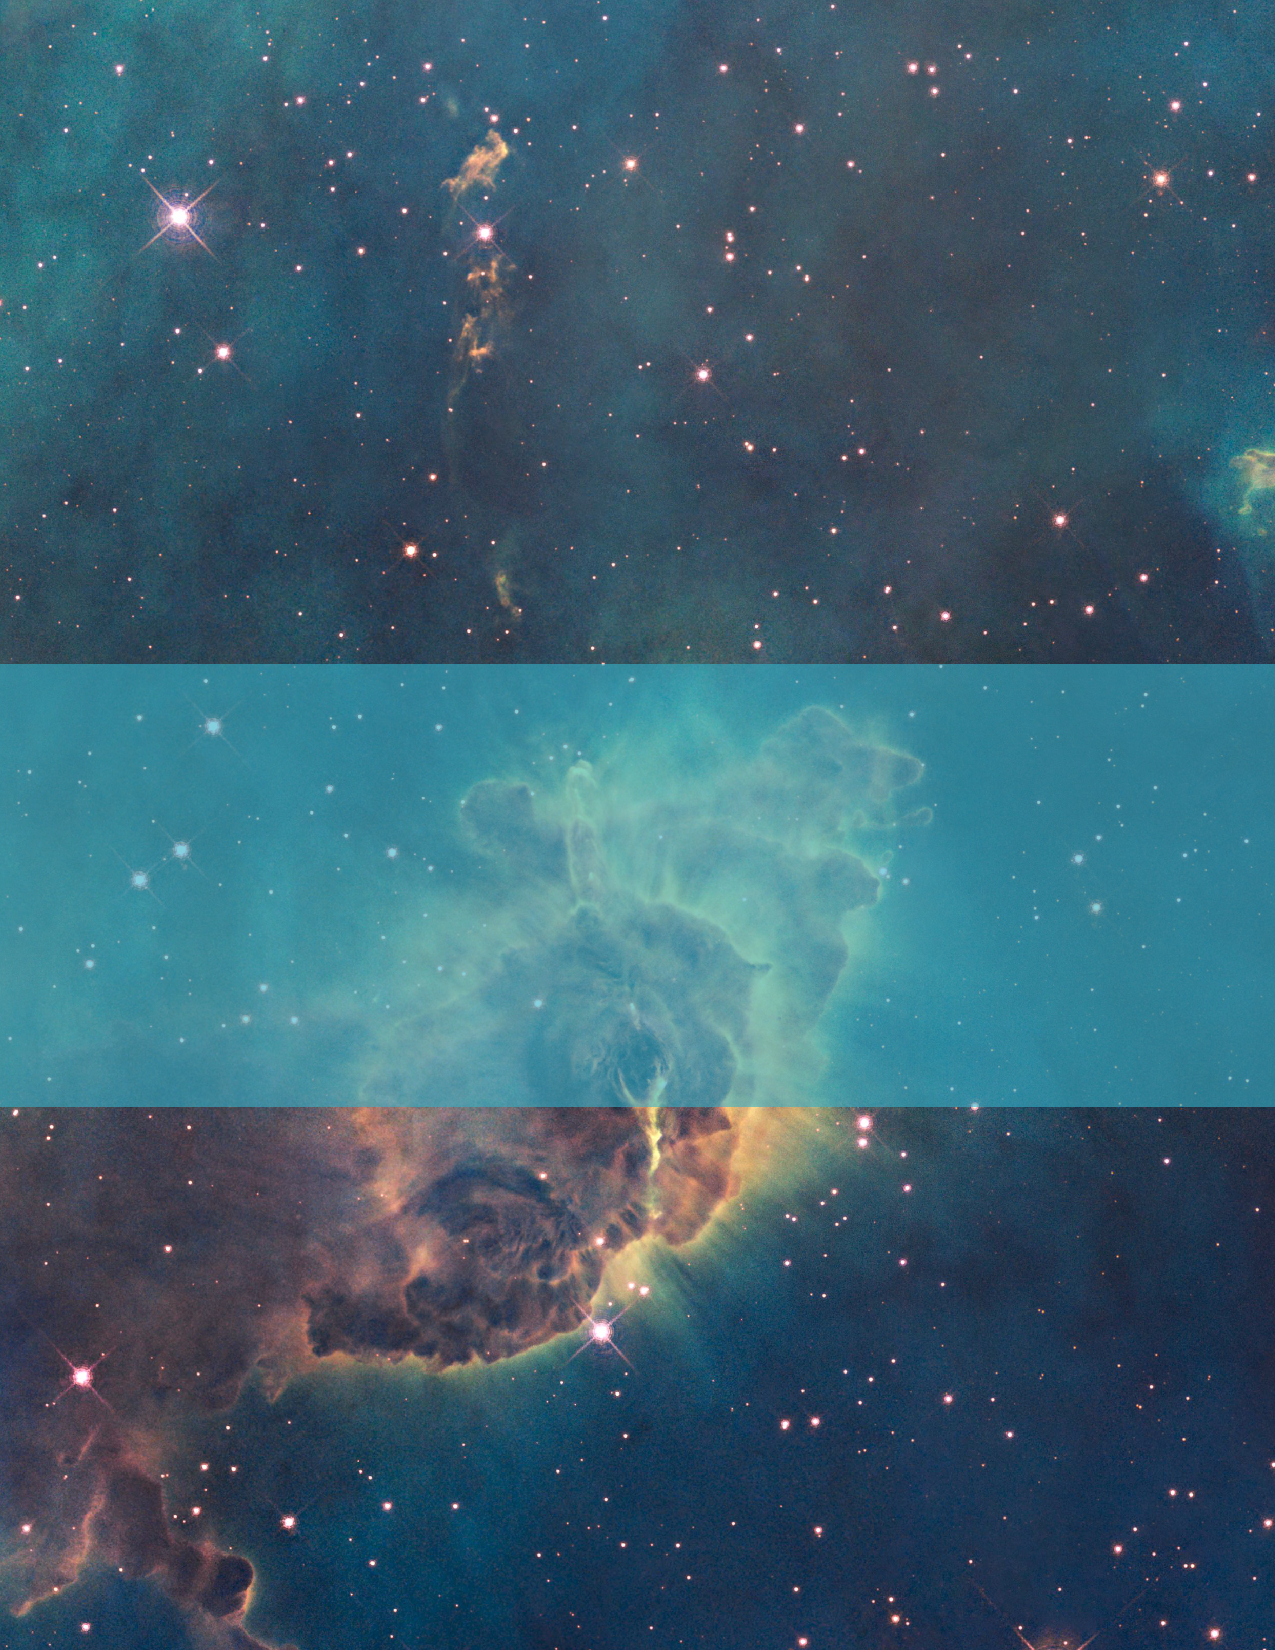
\includegraphics[scale=1.25]{esahubble}}} % Image background
\centering
\vspace*{5cm}
\par\normalfont\fontsize{35}{35}\sffamily\selectfont
\textbf{PRINCIPLES OF QUANTUM MECHANICS}\\
{\LARGE R. Shankar}\par % Book title
\vspace*{1cm}
{\Huge Lecture Notes}\par % Author name
\endgroup

%----------------------------------------------------------------------------------------
%	COPYRIGHT PAGE
%----------------------------------------------------------------------------------------

\newpage
~\vfill
\thispagestyle{empty}

%\noindent Copyright \copyright\ 2014 Andrea Hidalgo\\ % Copyright notice

\noindent \textsc{Notes from the book Principles of Quantum Mechanics.}
\vspace{\baselineskip}

\noindent These notes have been taking while self-studying the book Principles of Quantum Mechanics by R. Shankar, second edition.

\noindent \textit{First release, July 2022} % Printing/edition date

%----------------------------------------------------------------------------------------
%	TABLE OF CONTENTS
%----------------------------------------------------------------------------------------

\chapterimage{head1.png} % Table of contents heading image

\pagestyle{empty} % No headers

\tableofcontents % Print the table of contents itself

%\cleardoublepage % Forces the first chapter to start on an odd page so it's on the right

\pagestyle{fancy} % Print headers again

%----------------------------------------------------------------------------------------
%	CHAPTER 1
%----------------------------------------------------------------------------------------

\chapterimage{head2.png} % Chapter heading image
\chapter{Mathematical introduction}
\section{Vector spaces}
\begin{definition}[Group]
    A group is a set $G$ together with a binary operation here denoted "$\cdot$", that combines any two elements  $a$ and $b$ 
    to form an element of $G$, denoted $a\cdot b$, such that the following three requirements, known as group \textit{axioms}, 
    are satisfied
    \begin{enumerate}
        \item Associativity: $\forall\: a,b,c \in G\; (a\cdot b)\cdot c = a\cdot (b\cdot c)$.
        \item Identity: $\exists\: e \in G\;\mid\; \forall a\in G\; e\cdot a=a\cdot e=a$. 
        \item Inverse $\forall a\in G\;\exists\; a^{-1}\in G \mid a^{-1}\cdot a=a\cdot a^{-1}=e$.
    \end{enumerate}
\end{definition}

\begin{remark}
    In the definition of the identity and inverse element, we clearly stated that they commute with any element of the group. This is
    important to state in the defition, because the operation defined on the group is not necessarily commutative.    
\end{remark}

\begin{remark}
    From the assioms it follows that the identity element is unique. If $e$ and $f$ are both identity elements, then $e=e\cdot f=f$.
    
    Similarly, the inverse of an element $a$ of the group is also unique. If $a$ has both $a_1^{-1}$ and $a_2^{-1}$ as inverse, then
    $a_2^{-1} = a_2^{-1}\cdot e = a_2^{-1}\cdot(a\cdot a_1^{-1}) = (a_2^{-1}\cdot a)\cdot a_1^{-1}=e\cdot a_1^{-1}=a_1^{-1}$.
\end{remark}

\begin{definition}[Abelian group]
    A group is \textit{abelian} if the operation defined on it is commutative.
\end{definition}

\begin{definition}[Field]
    A field is a set $F$ together with two binary operations, called addition and multiplication; 
    it is an \textit{abelian} group under addition with $0$ as the additive identity; 
    the \textit{non zero} elements are an \textit{abelian} group under multiplication with $1$ as the multiplicative identity; 
    and multiplication distributes over addition: $\forall a,b\in F\; a\cdot(b+c)=(a\cdot b) + (a\cdot c)$.
\end{definition}

\begin{remark}
    $\R^2$ is a field with the multiplication defined by $(a,b)\cdot(c,d)=(ac-bd, ad+bc)$. This is exactly the multiplication of two
    complex numbers. Indeed, the complex numbers is the way to give $\R^2$ a field structure. For $n>2$ it is not possible to give $\R^n$
    the structure of a field. However, for $n=4$ we can have a pseudo field using the non-commutative quaternion multiplication.
    For $\R^8$ we can give up the associativity of the multiplication and get the non-associative Caley algebra (octanions).
\end{remark}

\begin{definition}[Vector space]
A vector space over a field $F$ is a set $V$ together with two binary operations. 
The first operation, called vector addition assigns to any two vectors $\ket{V}$ and $\ket{W}$ in $V$ a third vector in $V$ which is commonly written as $\ket{v+w}$.
The second operation, called scalar multiplication, assigns to any scalar $a$ in $F$ and any vector $\ket{V}$ in $V$ another vector in $V$, which is denoted $a\ket{V}$.
These two operations must satisfy the eight following axioms:
\begin{enumerate}
    \item Associativity of vector addition:
    $\forall\: \ket{U}, \ket{V}, \ket{W} \in V\; \ket{U}+(\ket{V}+\ket{W}) = (\ket{U}+\ket{V})+\ket{W}$.
    \item Commutativity of vector addition: $\forall\: \ket{U}, \ket{V} \in V\; \ket{U}+\ket{V}=\ket{V}+\ket{U}$.
    \item Identity element of vector addition:
    $\exists\: \ket{0}\in V\;\mid\;\forall \ket{V}\in V\;\ket{V} + \ket{0}= \ket{V}$. 
    \item Inverse elements of vector addition: $\forall \ket{V}\in V\;\exists\; \ket{-V}\in V \mid 
    \ket{V}+\ket{-V}=\ket{0}$.
    \item Compatibility of scalar multiplication with field multiplication:\\
    $\forall\: a,b\in F\: \ket{V}\in V\;a(b\ket{V}) = (ab)\ket{V}$.
    \item Identity element of scalar multiplication: if $1$ is the multiplicative identity in $F$, then $\forall\:\ket{V}\in V\;1\ket{V}=\ket{V}$.
    \item Distributivity of scalar multiplication with respect to vector addition: $\forall\: a\in F\:\ket{U},\ket{V}\in V\: a(\ket{U}+\ket{V})=a\ket{U}+a\ket{V}$.
    \item Distributivity of scalar multiplication with respect to field addition: 
    $\forall\: a,b\in F\:\ket{V}\in V\:(a+b)\ket{V} = a\ket{V}+b\ket{V}$.
\end{enumerate}
Subtraction of two vectors can be defined as $\ket{V}-\ket{W} = \ket{V} + \ket{-w}$.
\end{definition}

\begin{remark}
    From the axioms it follows that 
    \begin{enumerate}
        \item $\ket{0}$ and the inverse are unique. The proof is the same as for the case of the group above.
        \item $0\ket{V}=0$: $\ket{V}=1\ket{V}=(0+1)\ket{V}=0\ket{V}+\ket{V}\Rightarrow 0\ket{V}=0$.
        \item $\ket{-V}=-\ket{V}$
    \end{enumerate}
\end{remark}

\begin{example}
    Consider all functions $f(x)$ defined in an interval $0<x<L$ and such that $f(0)=f(L)=0$. 
    We define scalar multiplication by $a$ simply as $af(x)$ and addition as pointwise addition. These functions form a vector space where 
    $\ket{0}$ is the function which is zero everywhere and the additive inverse of $\ket{f(x)}$ is $\ket{-f(x)}$.
    Notice that if $f(0)=f(L)\neq 0$ then we do not have a vector space.
\end{example}

\subsection{Linear independency}
\begin{definition}[Linear independency]
    A set of vectors $\ket{i}$ is said to be linearly independent if
    $\sum a_i\ket{i}=\ket{0}$
    is satisfied only by the trivial solution $a_i=0$.
\end{definition}

\begin{remark}
    If a set of vectors is linearly dependent, there must exist at least two $a_i\neq 0$. Let's say $a_3\neq 0$, then
    $\ket{3}=-\sum_{i\neq 3}\frac{a_i}{a_3}\ket{i}$. That is, in a set of linearly dependent vectors, at least one of them
    can be written as a linear combination of the other. On the other hand, it is not possible to write any member of the
    linearly independent set in terms of the others.
\end{remark}

\begin{definition}[Dimension of the vector space]
    A vector space has dimension $n$ if it can accommodate a maximum
    of $n$ linearly independent vectors. It will be denoted by $V^n$.
\end{definition}

\begin{example}
    The set of $2 \times 2$ matrices is a four-dimensional vector space. In fact, the following four vectors are linearly indpenedent:
    \begin{equation*}
        \begin{array}{cccc}
            \ket{1}=\left[
                \begin{array}{cc}
                    1&0\\
                    0&0
                \end{array}
        \right] &
        \ket{2}=\left[
            \begin{array}{cc}
                0&1\\
                0&0
            \end{array}
        \right] &
        \ket{3}=\left[
            \begin{array}{cc}
                0&0\\
                1&0
            \end{array}
        \right] &
        \ket{4}=\left[
            \begin{array}{cc}
                0&0\\
                0&1
            \end{array}
        \right]
        \end{array}
    \end{equation*} 
    Notice that any other matrix can be written as a linear combination of these four matrices. We have seen that in a set of linearly
    independent vectors, no vector can be written as a linear combination of the others. This means that the four matrices given above 
    represent the largest set of linearly independent vectors, and the vector space of $2\times 2$ matrices has dimension $n=4$.
\end{example}

\begin{definition}[Basis]
    A set of $n$ linearly independent vectors in an $n$-dimensional space is called a \textit{basis}.
\end{definition}

\begin{definition}[Component]
    Given a basis $\ket{i}$, any vector $\ket{V}$ can be written as a linear combination of the vectors $\ket{i}$. The coefficients of the
    linear combination are called the \textit{components} of $\ket{V}$ in the basis $\ket{i}$.
\end{definition}

\begin{theorem}
    The expansion of a vector in a given basis is unique.
\end{theorem}
\begin{proof}
    Let's suppose that there exist two different expansions:
    \begin{equation*}
        \ket{V}=\sum a_i\ket{i} = \sum a'_i\ket{i}
    \end{equation*}
    It follows
    \begin{equation*}
        \sum a_i\ket{i} - \sum a'_i\ket{i} =  \sum (a_i-a'_i)\ket{i} = \ket{0}
    \end{equation*}
    Since $\ket{i}$ are linearly independent, this means that $a_i=a'_i$ and the expansion is unique.
\end{proof}

\subsection{Inner product space}
\begin{definition}[Inner product]
    The \textit{inner product} or \textit{scalar product} is an operation that takes two vectors $\ket{V}$ and $\ket{W}$ and
    returns a scalar, denoted $\scalar{W}{V}$ satisfying the following axioms:
    \begin{enumerate}
        \item Skew symmetry: $\scalar{W}{V}=\scalar{V}{W}^*$.
        \item Positive semidefiniteness: $\scalar{V}{V}\geq 0$ and the equality holds iff $\ket{V}=\ket{0}$.
        \item Linearity in the ket: $\bra{W}(a\ket{V}+b\ket{Z})=a\scalar{W}{V}+b\scalar{W}{Z}\equiv\scalar{W}{aV+bZ}$.
    \end{enumerate}
    A vector space together with an inner product is called \textit{inner product space}.
\end{definition}

\begin{remark}
    From the axioms of the inner product it follows:
    \begin{enumerate}
        \item $\scalar{V}{V}$ is a real non-negative number. Therefore, $\sqrt{\scalar{V}{V}}$ is well defined.
        \item Antilinearity with respect to the first factor: $\scalar{aW+bZ}{V}=a^*\scalar{W}{V}+b^*\scalar{Z}{V}$. 
    \end{enumerate}
\end{remark}

\begin{definition}[Norm and orthogonality]
    The \textit{norm} of a vector is defined as $|V|\equiv\sqrt{\scalar{V}{V}}$. 
    Two vectors $\ket{V}$ and $\ket{W}$ are \textit{orthogonal} if $\scalar{W}{V}=0$.
\end{definition}

\begin{remark}
    Orthogonal vectors are also linear independent. If $\ket{V}$ and $\ket{W}$ are orthogonal, let's consider
    $a\ket{V}+b\ket{W}=0$. Taking the inner product with $\ket{V}$ and using the orthogonality, we get $a=0$. Similarly, the
    inner product with $\ket{W}$ leads to $b=0$.
\end{remark}

\begin{definition}[Dual space and bras]
    Any ket $\ket{V}$ induces a linear function $\scalar{V}{\cdot}$ that associates to each ket $\ket{W}$ its inner product with 
    $\ket{V}$. The space of all linear functions $\scalar{V}{\cdot}$ generated by all vectors $\ket{V}$ of a vector space $V$ is
    is itself a vector space and is called the \textit{dual} of $V$. 
    The elements of the dual space are called \textit{bras} and denoted by $\bra{V}$.
\end{definition}

An inner product can take the form of any function satisfying the axioms. However, given an orthonormal basis, the inner product can be
expressed in an easy way in terms of the components of the vectors. Let $\ket{i}$ be an orthonormal basis, and let 
$\ket{V}=\sum v_i\ket{i}$ and $\ket{W}=\sum w_i\ket{i}$. Then, 
$\scalar{W}{V}=\sum_{i,j}w^*_iv_j\scalar{i}{j}=\sum_{i,j}w^*_iv_j\delta_{ij}=\sum_i w^*_iv_i$.
I.e., in an orthonormal basis, the inner product is just the sum of the products of the single components. However, which basis is 
orthonormal depends on the specific inner product chosen.

Notice that it is convention to write the components of a ket as a column vector.
So the inner product is a number we are trying to generate from two kets $\ket{V}$ and $\ket{W}$, which are both represented by column vectors
in some basis. Now there is no way to make a number out of two columns by direct matrix multiplication, but there is a way to make a number 
by matrix multiplication of a row times a column. In particular, if we represent the bra $\bra{W}$ with the \textit{adjoint} (transpose
conjugate) of $\ket{W}$, in an orthonormal basis we have 
\begin{equation}
    \label{eq:bra_components}
    \scalar{W}{V}=[w^*_1,...,w^*_n]
    \left[\begin{array}{c}
        v^1\\
        \vdots\\
        v^n
    \end{array}\right]=
    \sum_i w^*_iv^i\equiv w^*_iv^i
\end{equation}

\begin{remark}
    The components of the kets are written with lower indexes, while the components of a bra with higher indexes. We are also using Einstein's 
    convention to sum over reapeated up and down indexes. So an inner product is always expressed as the sum of up and low indexes.
\end{remark}

Let us now ask: if $\bra{V}$ is the bra corresponding to the ket $\ket{V}$ what bra corresponds to $a\ket{V}$ where $a$ is some scalar?
By going to any basis it is readily found that
\begin{equation*}
    a\ket{V}\rightarrow
    \left[\begin{array}{c}
        av_1\\
        av_2\\
        \vdots\\
        av_n
    \end{array}\right]
    \rightarrow [a^*v_1^*, a^*v_2^*, \dots,a^*v_n^*]\rightarrow\bra{V}a^*.
\end{equation*}
It is customary to write $a\ket{V}$ as $\ket{aV}$ and the corresponding bra as $\bra{aV}$. What we have found is that
\begin{equation}
    \label{eq:bra_components_2}
    \bra{aV}=\bra{V}a^*
\end{equation}

The inner product allows us to easily get the components of a vector in an orthonormal basis. Let $\ket{i}$ be an orthonormal basis, then
$\ket{V}=\sum v_i\ket{i}$.
Taking the inner product with a specific base vector $\ket{j}$ leads to $\scalar{j}{V}=v_j$ and therefore
\begin{equation}
    \ket{V}=\sum\ket{i}\scalar{i}{V}
\end{equation}

\begin{theorem}
    Any inner product satisfies two properties:
    \begin{enumerate}
        \item Schwarz inequality: $|\scalar{V}{W}|\leq|V||W|$.
        \item Triangle inequality: $|V+W|\leq|V|+|W|$.
    \end{enumerate}
    In both cases, the equality holds iif $\ket{V}$ and $\ket{W}$ are linearly dependent.
\end{theorem}
\begin{proof}
    For the Schwarz inequality, from
    \begin{equation*}
        \ket{Z}=\ket{V}-\frac{\scalar{W}{V}}{|W|^2}\ket{W}
    \end{equation*}
    we get
    \begin{equation*}
        0\leq\scalar{Z}{Z}=\scalar{V}{V}-\frac{\scalar{W}{V}\scalar{V}{W}}{|W|^2}
    \end{equation*}
    which leads to
    $|V|^2|W|^2\geq|\scalar{W}{V}|^2$ and therefore proves the Schwarz inequality.

    The proof for the triangle inequality is similar, starting with $|V+W|^2$ and considering $\mbox{Re}\scalar{V}{W}\leq|\scalar{V}{W}|$.
\end{proof}

\section{Linear operators}
An operator $\Omega$ is an instruction to transform a vector $\ket{V}$ into another vector $\ket{V'}$. This is represented by writing
$\Omega\ket{V}=\ket{V'}$.

\begin{definition}[Linear operator]
A \textit{linear operator} is an operator that satisfies
\begin{equation*}
    \Omega(\alpha\ket{V}+\beta\ket{W}) = \alpha\Omega\ket{V} + \beta\Omega\ket{W}
\end{equation*}
\end{definition}

\begin{remark}
    A nice feature of linear operators is that once their action on the basis vectors is known, their action on any vector in the space
    is determined. If we are given a basis $\ket{i}$ for our space, then the action of $\Omega$ on any vector $\ket{V}$ is given 
    by $\Omega\ket{V} = \sum v_i\Omega\ket{i}$
\end{remark}

The \textit{product of two operators} stands for the instruction that the action of the two operators be carried out in sequence.
Notice that the order of the operations matters, i.e., in general $\Omega\Lambda\neq\Lambda\Omega$. An example are rotations in 3D space.
\begin{definition}[Commutator]
    The commutator of two operators is defined as 
    \begin{equation*}
        [\Omega,\Lambda] = \Omega\Lambda-\Lambda\Omega
    \end{equation*}
\end{definition}

\begin{theorem}
    The commutator satisfies 
    \begin{equation}
        [\Omega, \Lambda\Theta] = \Lambda[\Omega, \Theta] + [\Omega, \Lambda]\Theta
    \end{equation}        
\end{theorem}
\begin{proof}
    Given a generic vector $\ket{V}$, we have
    \begin{equation*}
        [\Omega, \Lambda\Theta]\ket{V} = \Omega\Lambda\Theta\ket{V} - \Lambda\Theta\Omega\ket{V}
    \end{equation*}
Using the fact that $\Omega\Lambda = [\Omega,\Lambda]+\Lambda\Omega$ we can rewrite the previous equality as
\begin{equation*}
    [\Omega, \Lambda\Theta]\ket{V} = 
    [\Omega,\Lambda]\Theta\ket{V}+\Lambda\Omega\Theta\ket{V} - \Lambda\Theta\Omega\ket{V} =
    [\Omega,\Lambda]\Theta\ket{V} + \Lambda[\Omega,\Theta]\ket{V}
\end{equation*}
Since $\ket{V}$ is a generic vector, this equality must hold for all $\ket{V}\in V$.
\end{proof}

\begin{definition}
    The \textit{inverse} of $\Omega$, denoted by $\Omega^{-1}$, is defined such that $\Omega\Omega^{-1}=\Omega^{-1}\Omega=1$.
\end{definition}
\begin{remark}
    For linear operators acting on a vector space $V^n$ with $n$ finite, it can be shown that
    $\Omega\Omega^{-1}=1$ iif $\Omega^{-1}\Omega=1$.
\end{remark}
\begin{theorem}
    The inverse of a product of operators is given by
    \begin{equation}
        \left(\Omega\Lambda\right)^{-1} = \Lambda^{-1}\Omega^{-1}
    \end{equation}
\end{theorem}
\begin{proof}
    $\left(\Omega\Lambda\right)^{-1}$ is defined such that 
    \begin{equation*}
        \left(\Omega\Lambda\right)^{-1}\Omega\Lambda=1
    \end{equation*}
    If we multiply both sides by $\Lambda^{-1}$ to the right, we get 
    \begin{equation*}
        \left(\Omega\Lambda\right)^{-1}\Omega = \Lambda^{-1}
    \end{equation*}
    Multiplying both sides by $\Omega^{-1}$ to the right gives
    \begin{equation*}
        \left(\Omega\Lambda\right)^{-1} = \Lambda^{-1}\Omega^{-1}
    \end{equation*}
\end{proof}

\subsection{Matrix elements}
We have seen that an abstract vector can be represented in a basis by an n-tuple of numbers, called its components,
in terms of which all vector operations can be carried out.
We shall now see that in the same manner a linear operator can be represented in a basis by an $n\times n$
matrix.

Let's consider $\ket{V'}=\Omega\ket{V}$. In terms of the components on basis $\ket{i}$, this can be rewritten
\begin{equation*}
    \sum v'_i\ket{i} = \sum v_i\Omega\ket{i}
\end{equation*}
Taking the inner product with $\ket{j}$ of both sides gives an expression for $v'_j$
\begin{equation*}
    v'_j = v_j\bra{j}\Omega\ket{i}
\end{equation*}
And therefore
\begin{equation*}
    \sum v'_i\ket{i} = \sum v_j\bra{j}\Omega\ket{i}
\end{equation*}
If we define the matrix
\begin{equation}
    \label{eq:matrix_operator}
    \Omega^j\:_i\equiv \bra{j}\Omega\ket{i}
\end{equation}
We can write the transformed vector $\ket{V'}=\Omega\ket{V}$ as the matrix multiplication
\begin{equation}
    (v')^j=\Omega^j\:_iv^i    
\end{equation}
where we used the Einstein's sum convention.

\begin{remark}
    A mnemonic: the elements of the $i$-th column of $\Omega^j\:_i$ are simply the components of the $i$-th
transformed basis vector $\ket{i'}=\Omega\ket{i}$ in the given basis.
\end{remark}

\begin{example}
    \label{example:rotation_matrix}
    Let's consider rotations in 3D space, i.e. the operator $R\left(\frac{1}{2}\pi \hat i\right)$ that rotates
    a vector by $\frac{1}{2}\pi$ about the unit vector $\hat i$. Notice that this operator is linear.
    
    Let us consider the action of this operator on the three unit vectors $\hat i$, $\hat j$, and $\hat k$, which
    in our notation will be denoted by $\ket{1}$, $\ket{2}$, $\ket{3}$
    \begin{eqnarray*}
        \left(\frac{1}{2}\pi \hat i\right)\ket{1} &=& \ket{1} \\
        \left(\frac{1}{2}\pi \hat i\right)\ket{2} &=& \ket{3} \\
        \left(\frac{1}{2}\pi \hat i\right)\ket{3} &=& -\ket{2} \\
    \end{eqnarray*}

    Following our mnemonic, the matrix representation of $R\left(\frac{1}{2}\pi \hat i\right)$ is
    \begin{equation*}
        R\left(\frac{1}{2}\pi \hat i\right) \leftrightarrow \left[\begin{array}{ccc}
            1&0&0\\
            0&0&-1\\
            0&1&0
        \end{array}\right]
    \end{equation*}
\end{example}

\subsubsection{Projection operator}
We saw that a vector $\ket{V}$ can be expanded on a basis with the formula $\ket{V}=\sum\ket{i}\bra{i}\ket{V}$.
Each single term of the expansions, $\ket{V}=\ket{i}\bra{i}\ket{V}$ can be interpreted as a sort of projection of the 
vector onto the $i$-th basis vector. And this leads to the following definition
\begin{definition}[Projection operator]
    The operator $P_i = \ket{i}\bra{i}$ is a linear operator called the \textit{projection operator} for the ket $\ket{i}$.
\end{definition}
\begin{theorem}[Completeness]
    The projection operator satisfies the completeness relation, i.e., 
    \begin{equation}
        \label{eq:completness}
        \sum P_i =\sum\ket{i}\bra{i }= 1
    \end{equation}
\end{theorem}
\begin{proof}
    A generic vector $\ket{V}$ can be expanded on a basis using the projection operators
    \begin{equation*}
        \ket{V} = \sum P_i\ket{V} = \left(\sum P_i\right)\ket{V} 
    \end{equation*}
    Since $\ket{V}$ is a generic vector, it must hold that $\left(\sum P_i\right)=1$.
\end{proof}
\begin{remark}
    The completeness relation says that the sum of the projections of a vector along all the $n$
    directions equals the vector itself.
\end{remark}
\begin{remark}
    Pojection operators corresponding to the basis vectors obey $P_jP_i=\delta_{ij}$.
    This tells us that once $P_i$ projects out the part of $\ket{V}$ along $\ket{i}$, further applications of $P_i$, make
    no difference; and the subsequent application of $P_j$ with $j\neq i$ will result in zero, since a vector entirely
    along $\ket{i}$ cannot have a projection along a perpendicular direction $\ket{j}$.
\end{remark}

The matrix elements of $P_i$ are given by Eq. \ref{eq:matrix_operator}
\begin{equation*}
    \left(P_i\right)^k\:_l = \bra{k}P_i\ket{l} = \scalar{k}{l}\delta_{il} = \delta_{kl}\delta_{il} = \delta^k\:_i\delta_{il}
\end{equation*}
This matrix has $0$ everywhere, except for $1$ at position $(i,i)$. This is in agreement with our mnemonic that the matrix of a linear
operator contains per columns the components of the transformed basis vectors. In the case of the projection operator $P_i$, all base 
vectors except $\ket{i}$ gives $\ket{0}$. But the base vector $\ket{i}$  stays untrasformed.

The matrix also arises if we consider $\ket{i}\bra{i}$ component-wise. $\ket{i}$ is a column vector of length $n$, while $\bra{i}$ 
is a row vector of dimension $n$. Therefore, $\ket{i}\bra{i}$ is the multiplication of a $1\times n$ matrix with a $n\times 1$ matrix,
which gives the $n\times n$ matrix reported above.

\begin{remark}
    The completeness relation, Eq. \ref{eq:completness} says that when all the $P_i$ are added, the diagonal fills out to give the
    identity. If we form the sum over just some of the projection operators, we get the operator which projects a given vector into the 
    subspace spanned by just the corresponding basis vectors.
\end{remark}

\subsection{Adjoint of an operator}
We have seen the action of an operator on a ket $\ket{V}$. But what about the action on a bra $\bra{V}$?
In a given basis, we have seen that the bra is the transpose conjugate of the corresponding ket (see Eq. \ref{eq:bra_components}
and Eq. \ref{eq:bra_components_2}). Here will see that the same applies for operators.

\begin{definition}[Adjoint]
    If $\ket{\Omega}$ is the operator that turns a ket $\ket{V}$ into $\ket{V'}$, then its \textit{adjoint} $\Omega^\dagger$ is 
    defined as the operator that turns the bra $\bra{V}$ into $\bra{V'}$.
\end{definition}
\begin{theorem}
    In a given basis, the matrix representing $\Omega^\dagger$ is given by the transpose conjugate of the matrix
    representing $\Omega$.
\end{theorem}
\begin{proof}
    \begin{equation*}
        \left(\Omega^\dagger\right)_i\:^j = \bra{i}\Omega^\dagger\ket{j} = \scalar{\Omega i}{j} = \scalar{j}{\Omega i}^* = 
        \bra{j}\Omega\ket{i}^* = \left(\Omega^*\right)^j\:_i
    \end{equation*}
\end{proof}

\begin{theorem}
    The adjoint of a product is the product of the adjoints in reverse:
    \begin{equation}
        \left(\Omega\Lambda\right)^\dagger=\Lambda^\dagger\Omega^\dagger
    \end{equation}
\end{theorem}
\begin{proof}
    Let's consider $\bra{\Omega\Lambda V}$. First we treat $\Omega\Lambda$ as one operator and get
    \begin{equation*}
        \bra{\Omega\Lambda V} = \bra{V}\left(\Omega\Lambda\right)^\dagger
    \end{equation*}
    Next we treat $\Lambda$ and $\Omega$ as two distinct operators applied sequentially
    \begin{equation*}
        \bra{\Omega\Lambda V} = \bra{\Lambda V}\Omega^\dagger = \bra{V}\Lambda^\dagger\Omega^\dagger
    \end{equation*}
    Comparing the two equations and considering that $\ket{V}$ is a generic ket,
    we get the desired result $\left(\Omega\Lambda\right)^\dagger=\Lambda^\dagger\Omega^\dagger$.
\end{proof}


When a product of operators, bras, kets, and explicit numerical coefficients is encountered, reverse
the order of all factors and make the substitutions
\begin{eqnarray}
    \nonumber
    \Omega&\leftrightarrow&\Omega^\dagger
    \\
    \ket{V}&\leftrightarrow&\bra{V}
    \\\nonumber
    a&\leftrightarrow&a^*
\end{eqnarray}

\begin{example}
    Let's consider the following equation
    \begin{equation*}
        a_1\ket{V_1} = a_2\ket{V_2} + a_3\ket{V_3}\scalar{V_4}{V_5}+ a_4\Omega\Lambda\ket{V_6} 
    \end{equation*}
    Its adjoint is
    \begin{equation*}
        \bra{V_1}a^*_1 = \bra{V_2}a^*_2+ \scalar{V_4}{V_5}\bra{V_3}a^*_3+ \bra{V_6}\Lambda^\dagger\Omega^\dagger a_4^*
    \end{equation*}
    Of course, there is no real need to reverse the location of the scalars $a$ except in the interest of uniformity.
\end{example}

\begin{definition}[Hermitian and unitary  operators]
    An operator is called 
    \begin{enumerate}
        \item \textit{Hermitian} if $\Omega^\dagger=\Omega$.
        \item \textit{Anti-Hermitian} if $\Omega^\dagger=-\Omega$.
        \item \textit{Unitary} if $\Omega\Omega^\dagger=1$.
    \end{enumerate}
\end{definition}

\begin{remark}
    Hermitian and anti-Hermitian operators are the equivalent of pure real and pure imaginary complex numbers. Unitary operators
    are the equivalent of complex numbers of unit modulus $e^{i\theta}$.
\end{remark}

\begin{theorem}
    Unitary operators preserve the inner product between the vectors they act on.
\end{theorem}
\begin{proof}
    Let $\ket{V'_1}=U\ket{V_1}$ and $\ket{V'_2}=U\ket{V_2}$. Then 
    \begin{equation*}
        \scalar{V'_1}{V'_2} = \bra{V_1}U^\dagger U\ket{V_2} = \scalar{V_1}{V_2}
    \end{equation*}
\end{proof}

\begin{remark}
    Unitary operators are the generalizations of rotation operators from $V^3(\mathbb{R})$ to $V^3(\mathbb{C})$,
    for just like rotation operators in three dimensions, they preserve the lengths of vectors and their dot products. 
    In fact, on a real vector space, the unitarity condition becomes $U^\dagger=U^T$, which defines an orthogonal or
    rotation matrix.
\end{remark}

\subsubsection{Active and passive transformations}
Suppose we subject all the vectors in a space to a unitary transformation $\ket{V}\rightarrow U\ket{V}$.
The matrix elements of any operator $\Omega$ are transformed as 
\begin{equation*}
    \bra{W}\Omega\ket{V}\rightarrow \bra{UW}\Omega\ket{UV}=\bra{W}U^\dagger\Omega U\ket{V}
\end{equation*}
It is clear that we would obtain the same matrix if we left the vectors alone and subjected all operators
to the change
\begin{equation*}
    \Omega\rightarrow U^\dagger\Omega U
\end{equation*}
The first case is called \textit{active transformation}, while the second one \textit{passive transformation}.
Later we will see that the physics in quantum theory lies in the matrix elements of operators, and that active and
passive transformations provide us with two equivalent ways of describing the same physical transformation.

\subsection{The eigenvalue problem}
When some linear operator $\Omega$ acts on an arbitrary nonzero ket $\ket{V}$, the ket will suffer a nontrivial 
change, i.e., $\Omega\ket{V}$ will not be simply related to $\ket{V}$.
So much for an arbitrary ket. Each operator, however, has certain kets of its own, on which its action is simply
that of rescaling.
\begin{definition}[Eigenvalues and eigenkets]
    Given a linear operator $\Omega$, any ket $\ket{V}$, such that
    \begin{equation}
        \label{eq:eigenvalue}
        \Omega\ket{V}=\omega\ket{V}
    \end{equation}
is called an \textit{eigenket} of $\Omega$ with \textit{eigenvalue} $\omega$.
\end{definition}

We want now find a general approach to find all eigenvalues and eigenkets of a linear operator.

\begin{theorem}
    The condition for nonzero eigenvectors is
    \begin{equation}
        \det  \left(\Omega-\omega I\right) = 0
    \end{equation}
\end{theorem}
\begin{proof}
    We start by rewriting \ref{eq:eigenvalue} as 
\begin{equation*}
        \left(\Omega-\omega I\right)\ket{V}=\ket{0}
    \end{equation*}
    From which it follows
    \begin{equation*}
        \ket{V} = \left(\Omega-\omega I\right)^{-1}\ket{0}
    \end{equation*}
    If the operator $\left(\Omega-\omega I\right)$ is finite (i.e. its matrix elements are finite), there is now way it can
    act on the null vector to give a nonzero ket $\ket{V}$. So $\left(\Omega-\omega I\right)$ cannot be finite.
    To find under which conditions the operator is not finite, let's recall that the inverse of a matrix is given by
    \begin{equation*}
        M^{-1}=\frac{\mbox{cofactor}\,M^T}{\det\,M}
    \end{equation*}
    where the cofactor of a matrix $M$ is the matrix whose element $(i,j)$ is $(-1)^{i+j}M_{i,j}$, and $M_{i,j}$ is the $(i,j)$ minor,
    i.e., the determinant of $M$ with the $i$-th row and $j$-th column removed.

    It is clear that the cofactor is always finite if $M$ is finite. So the only possibility to have an non finite inverse matrix
    is that the determinant is zero. That is, $\det  \left(\Omega-\omega I\right) = 0$.
\end{proof}

\begin{theorem}
    Every operator in $V^n(\mathbb{C})$ has $n$ eigenvalues, not necessarily distinct.
\end{theorem}
\begin{proof}
    To find the eigenvalues, we need to set to zero the determinant of a $n\times n$ matrix. Since the determinant of a $n\times n$
    matrix is a polynomial of order $n$, the fundamental theorem of algebra tells us that it can be decomposed as 
    \begin{equation*}
        \det  \left(\Omega-\omega I\right) = (\omega_1-\omega)(\omega_2-\omega)\dots(\omega_n-\omega)=0
    \end{equation*}
    where the $\omega_i$ are not necessarily distinct. This equation has $n$ solutions in $\mathbb{C}$.
\end{proof}

\begin{example}
    Let's find the eigenvalues and eigenvectors of the rotation matrix. We saw in Example \ref{example:rotation_matrix} that the
    matrix representing a rotation of $pi/2$ around the x-axis is given by
    \begin{equation*}
        R\left(\frac{1}{2}\pi \hat i\right) \leftrightarrow \left[\begin{array}{ccc}
            1&0&0\\
            0&0&-1\\
            0&1&0
        \end{array}\right]
    \end{equation*}
    By setting the determinant to zero, we find $\omega=1,\,\pm i$. The eigenvalue $1$ has eigenvector $\ket{1}$. This means that a 
    vector aligned along $x$ doesn't change under a rotation around $x$. The complex values correspond to the vectors 
    \begin{equation*}
        \ket{\pm i} \rightarrow \frac{1}{\sqrt{2}}\left[\begin{array}{c}
            0\\
            \pm i\\
            0
        \end{array}\right]
    \end{equation*}
\end{example}

\subsubsection{Hermitian operators in $V^n(\mathbb{C})$}
\begin{theorem}
    The eigenvalues of an Hermitian operator are real.
\end{theorem}
\begin{proof}
    Let $\Omega\ket{\omega}=\omega\ket{\omega}$. It follows
    \begin{equation*}
        \bra{\omega}\Omega\ket{\omega}=\omega\scalar{\omega}{\omega}
    \end{equation*}
    The adjoint of this equation is
    \begin{equation*}
        \bra{\omega}\Omega^{\dagger}\ket{\omega}=\omega^*\scalar{\omega}{\omega}
    \end{equation*}
    But since $\Omega^{\dagger}=\Omega$, the previous two equations imply $\omega^*=\omega$.
\end{proof}

\begin{theorem}
    To every Hermitian operator $\Omega$, there exists (at least) a basis consisting of its orthonormal eigenvectors. It 
    is diagonal in this eigenbasis and has its eigenvalues as its diagonal entries.
\end{theorem}
\begin{proof}
    The characteristic equation must have at least one root, call it $\omega_1$. The corresponding eigenvector is $\ket{\omega_1}$.
    Consider the subspace $\mathbb{V}^{n-1}_{\perp 1}$ of all vectors orthogonal to $\ket{\omega_1}$. Let us choose as our basis
    $\ket{\omega_1}$ and any $(n-1)$ orthonormal vectors in $\mathbb{V}^{n-1}_{\perp 1}$. In this basis, $\Omega$ has the following
    form
    \begin{equation*}
        \Omega\leftrightarrow\left[\begin{array}{ccccc}
            \omega_1 &0 &0 &\dots&0\\
            0\\
            0\\
            \vdots\\
            0
        \end{array}\right]
    \end{equation*}
    The first column is simply the image of $\ket{\omega_1}$ under $\Omega$, while the first row comes from the hermiticity.
    The characteristic equation now takes the form
    \begin{equation*}
        (\omega-\omega_1)(\mbox{determinant of the minor $\Omega_{1,1}$})=0
    \end{equation*}
    The determinant of the minor is a polynomial and must generate one root, $\omega_2$ and a corresponding eigenvector $\ket{\omega_2}$.
    Define the subspace  $\mathbb{V}^{n-2}_{\perp 2}$ of all the vectors in  $\mathbb{V}^{n-1}_{\perp 1}$ orthogonal to $\ket{\omega_2}$, 
    and repeat the same procedure as before. Finally the matrix becomes, in the basis 
    $\ket{\omega_1},\,\ket{\omega_2},\,\ket{\omega_3},\,\dots,\,\ket{\omega_n}$
    \begin{equation*}
        \Omega\leftrightarrow\left[\begin{array}{ccccc}
            \omega_1 &0 &0 &\dots&0\\
            0 &\omega_2&0& \dots &0\\
            0 &0 &\omega_3& \dots &0\\
            \vdots&&&&\vdots\\
            0 &0&0& \dots &\omega_n\\
        \end{array}\right]
    \end{equation*}
    Since every $\ket{\omega_i}$ was chosen from a space that was orthogonal to the previous one, the vectors
    $\ket{\omega_1},\,\ket{\omega_2},\,\ket{\omega_3},\,\dots,\,\ket{\omega_n}$ are $n$ orthonormal vectors, i.e. a basis.
\end{proof}
In stating the previous theorem, it was indicated that there might exist more than one basis of eigenvectors that diagonalizes
$\Omega$. This happens if there is degeneracy. Suppose $\omega_1=\omega_2=\omega$. Then we have two orthonormal vectors obeying
\begin{eqnarray*}
    \Omega\ket{\omega_1} &=& \omega\ket{\omega_1} \\
    \Omega\ket{\omega_2} &=& \omega\ket{\omega_2}
\end{eqnarray*} 
It follows that 
\begin{equation*}
    \Omega\left[\alpha\ket{\omega_1}+\beta\ket{\omega_2}\right]=\omega\left[\alpha\ket{\omega_1}+\beta\ket{\omega_2}\right]
\end{equation*}
Since $ket{\omega_1}$ and $ket{\omega_2}$ are orthonormal, we find that there is a whole two-dimensional subspace, the elements
of which are eigenvectors of $\Omega$ with eigenvalue $\omega$. Therefore, besides $ket{\omega_1}$ and $ket{\omega_2}$ there exists an 
infinity of orthonormal pairs from which we may select any pair in forming the eigenbasis of $\Omega$.
Notice that in the face of degeneracy, $\ket{\omega_i}$ no longer refers to a single ket but
to a generic element of the eigenspace $\mathbb{V}^m_{\omega_i}$. To refer to a particular element, we must
use the symbol $\ket{\omega_i,\,\alpha}$, where $\alpha$ labels the ket within the eigenspace.
\begin{example}
    Let's find an orthonormal basis for 
    \begin{equation*}
        \Omega\leftrightarrow\left[\begin{array}{ccc}
            1 &0 &1\\
            0 &2&0\\
            1 &0 &1\\
        \end{array}\right]
    \end{equation*}
    The characteristic equation is $\omega(2-\omega)^2$, whose solutions are $\omega_1=2$ (with multiplicity 2), $\omega_2$=0.
    The eigenvector corresponding to $\omega_2=0$ is
    \begin{equation*}
        \ket{\omega=0}\leftrightarrow\frac{1}{\sqrt{2}}\left[
            \begin{array}{c}
                1\\
                0\\
                -1
            \end{array}\right]
    \end{equation*}
    For $\omega=2$ we have
    \begin{eqnarray*}
        x_1-x_3&=&0 \\
        0&=&0
    \end{eqnarray*}
    We now only have one equation for three variables and every vector of the form
    \begin{equation*}
        \left[\begin{array}{c}
            a\\
            b\\
            a
        \end{array}\right]
    \end{equation*}
    is an eigenvector orthogonal to $\ket{\omega=0}$. To form an orthonormal basis where $\Omega$ is diagonal, we can e.g. choose
    \begin{equation*}
        \ket{\omega=2,\,1}\leftrightarrow\frac{1}{\sqrt{3}}
        \left[\begin{array}{c}
            1\\
            1\\
            1
        \end{array}\right]
    \end{equation*}
    and
    \begin{equation*}
        \ket{\omega=2,\,2}\leftrightarrow\frac{1}{\sqrt{6}}
        \left[\begin{array}{c}
            1\\
            -2\\
            1
        \end{array}\right]
    \end{equation*}
    However, any two vectors belonging to the subspace spanned by $\ket{\omega=2,\,1}$ and $\ket{\omega=2,\,2}$ can be chosen to form
    an orthonormal basis together with $\ket{\omega=0}$.
\end{example}
\begin{theorem}
    Every Hermitian matrix on $\mathbb{V}^n(\mathbb{C})$ can be diagonalized by a unitary change of basis. Equivalently,
    If $\Omega$ is a Hermitian matrix, there exists a unitary matrix $U$ (built out of the eigenvectors of $\Omega$) such that 
    $U^\dagger\Omega U$ is diagonal.
\end{theorem}
\begin{proof}
    Consider a Hermitian operator $\Omega$ on $\mathbb{V}^n(\mathbb{C})$ represented as a matrix in some
    orthonormal basis $\ket{1}\,,\ket{2}\,,\dots,\,\ket{n}$. If we trade this basis for the eigenbasis
    $\ket{\omega_1}\,,\ket{\omega_2}\,,\dots,\,\ket{\omega_n}$, the matrix representing $\Omega$ will become diagonal. 
    Now the operator $U$ inducing the change of basis $\ket{\omega_i}=U\ket{i}$ is unitary, because its matrix contains by
    columns the components of the eigenvectors $\ket{\omega_i}$ that are orthonormal.
\end{proof}
\begin{theorem}
    If $\Omega$ and $\Lambda$ are two commuting Hermitian operators, there exists (at least) a basis of common eigenvectors that 
    diagonalizes them both.
\end{theorem}
\begin{proof}
    We will show the proof only in the case one of the two operators is not degenerate. However, the theorem holds also in case both 
    operators are degenerate.

    Let's suppose $\Omega$ is not degenerate, i.e. to a given eigenvalue there is only one eigenvector, up to a scale factor. Consider
    one of its eigenvector
    \begin{equation*}
        \Omega\Lambda\ket{\omega}=\Lambda\Omega\ket{\omega}=\omega\Lambda\ket{\omega}
    \end{equation*}
    That is, $\Lambda\ket{\omega}$ is an eigenvector of $\Omega$ with eigenvalue $\omega$. But since $\Omega$ is not degenerate,
     $\Lambda\ket{\omega}$ must be proportional to $\ket{\omega}$, i.e. $\Lambda\ket{\omega}=\lambda\ket{\omega}$.
     Since every eigenvector of $\Omega$ is also eigenvector of $\Lambda$, the basis $\ket{\omega_i}$ diagonalizes also $\Lambda$.
\end{proof}
\begin{remark}
    Here is an intuitive argument of what happens if $\Omega$ and $\Lambda$ are both degenerate.

    If $\Omega$ and $\Lambda$ are both degenerate, there exists a subspace of dimension $m\leq n$ where each vector is an eigenvector of
    $\Omega$ with eigenvalue $\omega$ and any set of $m$ orthonormal vectors will diagonalize $\Omega$. In this subspace,
    $\Lambda$ is still Hermitian, and, if restricted to this subspace, it is not degenerate, we can choose the set of $m$ eigenvectors such 
    that they are distinct eigenvectors of $\Lambda$, i.e. they are of the form $\ket{\omega,\,\lambda_i}$. 
    Thus, $\Lambda$ removes the ambiguity in choosing an eigenbasis.

    If in one of these subspaces $\Lambda$ is also degenerate, then we cannot entirely remove the ambiguity. But we might find a third 
    operator $\Gamma$ that commutes with $\Omega$ and $\Lambda$ and that is not degenerate. In this case the eigenvectors will have the 
    form $\ket{\omega,\,\lambda,\,\gamma_i}$.
\end{remark}

\subsubsection{Classical coupled harmonic oscillator}
Consider two equal masses $m$ linked by a spring of elastic constant $k$. Each mass is also connected to e rigid wall with a spring of 
constant $k$. If we call $x_1(t)$ and $x_2(t)$ the displacement of the two masses from their equilibrium positions, we see that
\begin{subequations}
    \label{eq:classic_ho_diff_eq}
    \begin{eqnarray}
        \ddot{x}_1(t) &=& -2\frac{k}{m}x_1(t) + \frac{k}{m}x_2(t) \\
        \ddot{x}_2(t) &=& -2\frac{k}{m}x_2(t) + \frac{k}{m}x_1(t)
    \end{eqnarray}
\end{subequations}
This equation can be written in matrix form
\begin{equation}
    \label{eq:classic_ho_diff_eq_vect}
    \ket{\ddot{x}(t)} = \Omega\ket{x(t)}
\end{equation}
Let's consider the basis vectors $\ket{1}$ and $\ket{2}$, where $\ket{x(t)}$ is given by $\left[x_1(t),\,x_2(t)\right]$. Then
\begin{equation*}
    \ket{x(t)} = \scalar{1}{x(t)}\ket{1} + \scalar{2}{x(t)}\ket{2} = x_1(t)\ket{1} + x_2(t)\ket{2}
\end{equation*}
If $x_2(t)=0$ and $x_1(t)=1$, then $\ket{x(t)} = \ket{1}$. Therefore, the two basis vectors have the following physical significance
\begin{eqnarray*}
    \ket{1}&\leftrightarrow&\left[\begin{array}{c}
        1\\
        0
    \end{array}\right] \leftrightarrow\left[\begin{array}{c}
        \mbox{first mass displaced by unity}\\
        \mbox{second mass undisplaced}
    \end{array}\right]
    \\
    \ket{2}&\leftrightarrow&\left[\begin{array}{c}
        0\\
        1
    \end{array}\right] \leftrightarrow\left[\begin{array}{c}
        \mbox{first mass undisplaced}
        \\
        \mbox{second mass displaced by unity}
    \end{array}\right]
\end{eqnarray*}
Eqs (\ref{eq:classic_ho_diff_eq}) are obtained by projecting Eq (\ref{eq:classic_ho_diff_eq_vect}) on the basis $\ket{1}$ and $\ket{2}$. In this basis, 
$\Omega$ is represented by the matrix
\begin{equation*}
    \Omega = \left[
        \begin{array}{cc}
            -2\omega^2 & \omega^2\\
            \omega^2 & -2\omega^2
        \end{array}
    \right]
\end{equation*}
where $\omega^2 = \frac{k}{m}$. 

Notice that $\Omega$ is Hermitian, therefore it exists a basis $\ket{I}$ and $\ket{II}$ where the operator is diagonal, making it easier to solve the 
system of differential equations.
The components of these basis vectors in the basis $\ket{1}$ and $\ket{2}$ is
\begin{subequations}
    \begin{eqnarray}
        \ket{I} &=& \frac{\ket{1}+\ket{2}}{\sqrt{2}} \\
        \ket{II} &=& \frac{\ket{1}-\ket{2}}{\sqrt{2}}
    \end{eqnarray}
\end{subequations}
corresponding to the eigenvalues $\omega_I^2=\omega^2$ and $\omega_{II}^2 = 3\omega^2$, respectively. In this basis, $\Omega$ is diagonal
\begin{equation*}
    \Omega = \left[
        \begin{array}{cc}
            \omega_I^2 & 0\\
            0 & \omega_{II}^2
        \end{array}
    \right]
\end{equation*}
In the new basis we lose the physical interpreatation of the single components, but the time evolution (\ref{eq:classic_ho_diff_eq_vect}) is given
by two decoupled differential equations. The solutions with null initial velocities are:
\begin{equation*}
    \begin{array}{cc}
        x_i(t) = x_i(0)\cos(\omega_i t), & i=I,II
    \end{array}
\end{equation*}
or, in vector form
\begin{equation*}
    \ket{x(t)} = \scalar{I}{x_0}\cos(\omega_I t)\ket{I} + \scalar{II}{x_0}\cos(\omega_{II} t)\ket{II} = 
    U\ket{x_0}
\end{equation*}

\begin{definition}[Propagator]
    The matrix
    \begin{equation*}
        U = \ket{I}\bra{I}\cos(\omega_I t) + \ket{II}\bra{II}\cos(\omega_{II} t)
    \end{equation*}
    is called the \textit{propagator}, because it propagates the initial state $\ket{x_0}$ to a state at a later time $\ket{x(t)}$.
\end{definition}
To find the time evolution of $\ket{x(t)}$ in the physical base, we simply needs to express the propagator on the basis $\ket{1}$ and $\ket{2}$
\begin{equation*}
    U \leftrightarrow \frac{1}{2}\left[
        \begin{array}{cc}
            \cos(\omega_I t)+\cos(\omega_{II} t) & \cos(\omega_I t)-\cos(\omega_{II} t) \\
            \cos(\omega_I t)-\cos(\omega_{II} t) & \cos(\omega_I t)+\cos(\omega_{II} t) \\
        \end{array}
    \right]
\end{equation*}
Finally
\begin{equation*}
    \left[\begin{array}{c}
        x_1(t) \\
        x_2(t)
    \end{array}\right] = 
    \left[\begin{array}{c}
        \frac{x_1(0)+x_2(0)}{2}\cos\left(\sqrt{\frac{k}{m}}\,t\right) + \frac{x_1(0)-x_2(0)}{2}\cos\left(\sqrt{\frac{3k}{m}}\,t\right) \\
        \frac{x_1(0)+x_2(0)}{2}\cos\left(\sqrt{\frac{k}{m}}\,t\right) - \frac{x_1(0)-x_2(0)}{2}\cos\left(\sqrt{\frac{3k}{m}}\,t\right)
    \end{array}\right]
\end{equation*}

The propagator depends only on the eigenvalues of the operator, but not on the initial state. This leads us to the following algorithm to 
solve a linear differential equation in the form $\ket{\ddot{x}(t)} = \Omega\ket{x(t)}$
\begin{enumerate}
    \item Find the eigenvalues and eigenvectors of $\Omega$.
    \item Construct the propagator $U$ in terms of the eigenvalues and eigenvectors.
    \item Compute the solution as $\ket{x(t)} = U\ket{x(0)}$.
\end{enumerate}

\begin{remark}
    The central problem in quantum mechanics is very similar to the simple example
    that we have just discussed. The state of the system is described in quantum theory
    by a ket $\ket{\psi}$ which obeys the Schr\"odinger equation $i\hbar\ket{\dot\psi}=H\ket{\psi}$. The algorithm to solve this equation is
    then to solve the eigenvalue problem for $H$ and build the propagator (following some rules).
\end{remark}

There are two initial states for which the dynamics is very simple. These are simply the eigenvectors $\ket{I}$ and $\ket{II}$. Indeed, if we start from 
$\ket{I}$ we get $\ket{x(t)} = \cos(\omega_I t)\ket{I}$. So in this case both components of the initial state oscillate with the same frequency, i.e. 
$x_1(t)$ and $x_2(t)$ move in synchronous. The same thing applies if we started from $\ket{x(0)} 0 \ket{II}$.

\begin{definition}[Normal mode]
    A motion in which all parts of the system move sinusoidally with the same frequency and with a fixed phase relation is called \textit{normal mode}.
\end{definition}

The pysical meaning of these two initial states is clear if we consider their projection on the physical basis $\ket{1}$ and $\ket{2}$. 
$\ket{I}$ corresponds to the masses being displaced by the same amount. In this case the middle spring is niether compressed or elongated and therefore doesn't
exert any force. The two masses oscillates only due to the force of the side springs, i.e., they oscillate with a frequency $k/m$. 
$\ket{II}$ corresponds to the two masses being displaced by the same but opposite amount. In this case the middle spring is distorced by double the amount, i.e. $2\Delta$.
Each mass is the subjected to a force from the lateral spring displaced by $\Delta$ and from the middle spring displaced by $2\Delta$, resulting in an oscillation 
frequency of $3k/m$.

\subsection{Functions of operators}
Functions on operators are defined based on their power expansion, under the assumption that the series converges to a definite limit.
For example consider $\exp{\Omega} = \sum_{n=0}^{\infty}\frac{\Omega^n}{n!}$. If $\Omega$ is Hermitian, we can always find an eigenbasis, and series becomes
\begin{equation*}
    e^\Omega=\left[
        \begin{array}{cccc}
            \sum_{m=0}^{\infty}\frac{\omega_1^m}{m!} &0 &\dots &0 \\
            0 &\sum_{m=0}^{\infty}\frac{\omega_2^m}{m!} &\dots &0 \\
            \dots &\dots &\dots &\dots \\
            0 &0 &\dots &\sum_{n=0}^{\infty}\frac{\omega_n^n}{n!}
        \end{array}
    \right] = 
    \left[
        \begin{array}{cccc}
            e^{\omega_1} &0 &\dots &0 \\
            0 &e^{\omega_2} &\dots &0 \\
            \dots &\dots &\dots &\dots \\
            0 &0 &\dots &e^{\omega_n}
        \end{array}
    \right]
\end{equation*}
So $e^\Omega$ is well defined in this basis, and therefore in any other basis.
\begin{remark}
    If $\Omega$ is Hermitian, $e^{i\Omega}$ is unitary. This is an analogy with the
    complex numbers: if $\theta$ is real, $e^{i\theta}$ has modulus one. 
\end{remark}

\begin{definition}[Derivative of an operator]
    If an operator $\Gamma(\lambda)$ depends on a parameter $\lambda$, we can define its derivative as
    \begin{equation*}
        \frac{d\Gamma}{d\lambda} = \lim_{\Delta\lambda\to 0}\frac{\Gamma(\lambda+\Delta\lambda) - \Gamma(\lambda)}{\Delta\lambda}
    \end{equation*}
    If $\Gamma(\lambda)$ is written as a matrix in some basis, then the matrix representing $\frac{d\Gamma}{d\lambda}$ is obtained
    by differentiating its matrix elements.
\end{definition}
A special case of $\Gamma(\lambda)$ we are interested in is $e^{\lambda\Omega}$, with $\Omega$ Hermitian. By going to the eigenbase of $\Omega$
we can show that
\begin{equation*}
    \frac{d e^{\lambda\Omega}}{d\lambda} = e^{\lambda\Omega}\Omega
\end{equation*}
Conversely, we can say that if we are confronted with the differential equation
\begin{equation*}
    \frac{d\Gamma}{d\lambda} = \Gamma\Omega
\end{equation*}
the solution is 
\begin{equation*}
    \Gamma(\lambda) = C e^{\lambda\Omega}
\end{equation*}

\begin{remark}
    In all the above examples, the operator behaved like if it were just a scalar. Now, the real difference between operators and scalars is that 
    operators might not commute. If only one operator is involved, everything commute and we can treat them as scalars. If, on the other hand, more
    than one operator in involved, the order of factors is important. For example, it is true that 
    \begin{equation*}
        e^{\alpha\Omega}e^{\beta\Omega} = e^{(\alpha+\beta)\Omega}
    \end{equation*}
    while it is not true that 
    \begin{equation*}
        e^{\alpha\Omega}e^{\alpha\Gamma} = e^{\alpha(\Omega+\Gamma)}
    \end{equation*}
    or
    \begin{equation*}
        e^{\alpha\Omega}e^{\beta\Gamma}e^{-\alpha\Omega} = e^{\beta\Gamma}
    \end{equation*}
    unless $\Omega$ and $\Gamma$ commute.
\end{remark}
\begin{theorem}
    In differentiating a product of operators, the chain rule is
    \begin{equation*}
        \frac{d}{d\lambda}e^{\lambda\Omega}e^{\lambda\Gamma} = \Omega e^{\lambda\Omega}e^{\lambda\Gamma} + e^{\lambda\Omega}e^{\lambda\Gamma}\Gamma
    \end{equation*}
    Notice how $\Omega$ appears to the left, while $\Gamma$ is on the right.
\end{theorem}
\begin{proof}
    Simply use the power series expansion.
\end{proof}

\subsection{Generalization to inifinite dimensions}
As an example of an infinite dimensional vector, consider a function defined in some interval $a\leq x\leq b$ and such that $f(x)=0$ at the 
boundary of the interval. The specification of the function is its value at any point $x$ in the interval. We can interpret the function $f$ 
as a ket $\ket{f}$, whose components are the value $f(x)$ the function assumes at every $a\leq x\leq b$. This vector is infinite dimensional. 

For $f$ to belong to a vector space, we need to define a sum and an inner product. The sum $\ket{f} + \ket{g}$ can be defined as the pointwise 
sum of the values of the two functions for each $x$. Since the functions vanish at the boundary of the interval, their sum also vanishes, therefore
$\ket{f} + \ket{g}$ still belongs to the space.
The inner product can be defined as
\begin{equation*}
    \scalar{f}{g}\equiv\int_a^b\!dx\, f(x)^*g(x)
\end{equation*}

In the discrete case, any vector $\ket{V}$ can be expanded on an orthonormal basis $\ket{i}$ as $\ket{V} = \sum \ket{i}\scalar{i}{V}$.
This generalizes in the continuous case. If we have an orthonormal basis $\ket{x}$, then
\begin{equation*}
    \ket{f} = \int_a^b\!dx\,\ket{x}\scalar{x}{f}
\end{equation*}
It follows that the completeness relation becomes
\begin{equation*}
    \int_a^b\!dx\,\ket{x}\bra{x}=1
\end{equation*}

\subsubsection{Orthonormal basis}
What are the basis vectors such that the components of $\ket{f}$ are the values $f(x)$ at every $x$? In the discrete case, the $i$-th basis vector would have
all the components $0$, except the $i$-th component which is $1$. In the infinite case, let's call $\ket{x}$ one such base vector,
we must have that $\scalar{x}{f}=\int_a^b\!dx'\, \scalar{x'}{x}f(x') = f(x)$. This can happen only if in this base 
\begin{equation*}
    \scalar{x'}{x} = \delta(x-x')    
\end{equation*}
That means, the components of a basis vector $\ket{x'}$ in the $\ket{x}$ basis are $\delta(x-x')$. The previous relation also represents the generalization of 
orthonormality to an infinite-dimensional vector space.

\begin{remark}
    Strictly speaking, the delta function is not a function, but a distribution. It has a meaning only inside an integral. Indeed, 
    in order to cancel out in the integral all contributions from $f(x')$ except $x'=x$, $\delta(x-x')$ must satisfy
    \begin{equation*}
        \delta(x-x') = \left\{\begin{array}{cc}
            0 & x\neq x' \\
           +\infty & x=x'
        \end{array}\right.
    \end{equation*}
    (for $x'=x$, the delta must be infinite, because the integral of any finite function that is different from zero only in countable many points is null).
    Moreover, it must satisfy
    \begin{equation*}
        \int_{-\infty}^{+\infty}\!dx'\,\delta(x-x') = 1
    \end{equation*}
    However, no function defined on the real numbers has these properties.
\end{remark}

\begin{theorem}[Derivative of the $\delta$]
    The derivative of the delta function over the first argument (the one not integrated over) is:
    \begin{equation*}
        \frac{d\delta}{dx}(x-x') = \delta(x-x')\frac{d}{dx}
    \end{equation*}
    Over the second argument (the one integrated over) we get a minus sign
    \begin{equation*}
        \frac{d\delta}{dx'}(x-x') = -\delta(x-x')\frac{d}{dx'}
    \end{equation*}
\end{theorem}
\begin{proof}
    The $\delta$ is defined only inside integrals, while acting of functions. The derivative over the first argument is
    \begin{equation*}
        \int\!dx'\,\frac{d\delta}{dx}(x-x')f(x') = \frac{d}{dx}\int\!dx'\,\delta(x-x')f(x') = \frac{d}{dx}f(x)
    \end{equation*}
    For the second argument we can use integration by parts to find
    \begin{equation*}
        \int\!dx'\,\frac{d\delta}{dx'}(x-x')f(x') =  \delta(x-x')f(x')\vert_a^b - \int\!dx'\ \delta(x-x')\frac{df}{dx'}(x')
    \end{equation*}
    Where the surface term vanishes since the $\delta$ function is null.
\end{proof}
In general, while deriving over the first term, it holds
\begin{equation*}
    \frac{d^n\delta}{dx^n}(x-x') =\delta(x-x')\frac{d^n}{x^n}
\end{equation*}


\begin{theorem}[Exponential representation of the delta function]
    The $\delta$ function can be represented as
    \begin{equation*}
        \delta(x-x') = \frac{1}{2\pi}\int_ {-\infty}^{+\infty}\!dk\,e^{ik(x'-x)}
    \end{equation*}
\end{theorem}
\begin{proof}
    Let's consider the Fourier transform of $f(x)$
    \begin{equation*}
        f(k) = \frac{1}{\sqrt{2\pi}}\int_ {-\infty}^{+\infty}\!dx\,e^{-ikx}f(x)
    \end{equation*}
    end its inverse
    \begin{equation*}
        f(x) = \frac{1}{\sqrt{2\pi}}\int_ {-\infty}^{+\infty}\!dk\,e^{ikx}f(k)
    \end{equation*}
    Then we can write
    \begin{equation*}
        f(x) = \int_ {-\infty}^{+\infty}\!dx'\,\left(\frac{1}{2\pi}\int_ {-\infty}^{+\infty}\!dk\,e^{ik(x'-x)}\right)f(x')
    \end{equation*}
    which means
    \begin{equation*}
        \frac{1}{2\pi}\int_ {-\infty}^{+\infty}\!dk\,e^{ik(x'-x)} = \delta(x-x')
    \end{equation*}
\end{proof}


\subsection{Derivative operator}
An example of an infinite dimensional operator is the derivative
\begin{equation*}
    D\ket{f} = \ket{\frac{d}{dx}f(x)}
\end{equation*}

Let's find the matrix representation $D_{xx'} \equiv \bra{x}D\ket{x'}$.
\begin{equation*}
     \bra{x}D\ket{f} = \scalar{x}{\frac{d}{dx}f(x)} = 
     \int\!\!dx'\,\bra{x}D\ket{x'}\scalar{x'}{f}dx' = 
     \int\!\!dx'\,\bra{x}D\ket{x'}f(x')dx'
\end{equation*}
From which it follows
\begin{equation}
    \label{eq:hermiticity_D}
    \bra{x}D\ket{x'} = \delta(x-x')\frac{d}{dx} = \delta'(x-x')
\end{equation}

\subsubsection{Hermiticity}
The derivative operator is not Hermitian
\begin{equation*}
    D_{x'x}^* = D_{x'x} = \delta'(x'-x) = -\delta'(x-x') = -D_{xx'} 
\end{equation*}
We can convert $D$ into an Hermitian matrix if we define $K\equiv -iD$. However, in an infinite dimensional space a 
Hermitian matrix is not guaranteed to correspond to a Hermitian operator.
Indeed, if $K$ is Hermitian, then $\bra{g}K\ket{f} = \bra{f}K\ket{g}^*$. Introducing some completenesses:
\begin{equation*}
    \int_a^b\!\!dx\,\int_a^b\!\!dx'\,\scalar{g}{x}\bra{x}K\ket{x'}\scalar{x'}{f}  = 
    \left[\int_a^b\!\!dx\,\int_a^b\!\!dx'\,\scalar{f}{x}\bra{x}K\ket{x'}\scalar{x'}{g} \right]^*
\end{equation*}
Replacing the matrix elements of $K$ with $K_{xx'} = \delta'(x-x')$ and integrating the left hand side by parts, we get
\begin{equation*}
    -ig^+(x)f(x)\vert_a^b + i\int_a^b\!\!dx\,\frac{dg^*}{dx}f(x) = i\int_a^b\!\!dx\,\frac{dg^*}{dx}f(x)
\end{equation*}
Therefore, the operator $K$ is Hermitian if and only if the surface term $-ig^+(x)f(x)\vert_a^b $ vanishes.
\begin{remark}
    In contrast to the finite-dimensional case, $K_{xx'} = K_{x'x}$ is not a sufficient condition for
    $K$ to be Hermitian. One also needs to look at the behavior of the functions at the end points a and b. 
\end{remark}
In quantum mechanics, we will be interested in functions defined over the full interval $-\infty<x<\infty$. 
Moreover, these functions will fall into two classes based on their behavior at $|x|\to\infty$: 
the functions that vanish, and the functions behaving as $e^{ikx}$.
If we consider matrix elements of $K$ between two functions of the first class, or one function of the first class and
one of the second class, the surface term disappears. The matrix elements between two functions of the second class gives
a surface term 
\begin{equation*}
    e^{-ik'x}e^{ikx}\vert_{-\infty}^{\infty}
\end{equation*}
If $k=k'$ the surface term vanishes. But if $k\neq k'$, the behavior is unclear, since $e^{-ik(x'-x)}$ oscillates without
reaching a limit for $|x|\to\infty$. Now, there exists a way of defining a limit for such functions that cannot make up
their minds: the limit as $|x|\to\infty$ is defined to be the average over a large interval. Following this prescription
\begin{equation*}
    \lim_{x\to\infty}e^{i(k-k')x} = 
    \lim_{\substack{L\to\infty\\\Delta\to\infty}}\frac{1}{\Delta}\int_L^{L+\Delta}\!\!dx\,e^{i(k-k')x} =
    \frac{e^{i(k-k')\Delta}}{i(k-k')}    
\end{equation*}
and
\begin{equation*}
    \lim_{x\to-\infty}e^{i(k-k')x} = 
    \lim_{\substack{L\to\infty\\\Delta\to\infty}}\frac{1}{\Delta}\int_{-L-\Delta}^{-L}\!\!dx\,e^{i(k-k')x} =
    \frac{e^{i(k-k')\Delta}}{i(k-k')}
\end{equation*}

Therefore, the surface term vanishes also in this case, and in the space relevant for quantum mechanics, $K$ is Hermitian.

\subsubsection{Eigenvectors and eigenvalues}
The eigenvalues and eigenvectors of $K$ are defined as
\begin{equation*}
    K\ket{k} = k\ket{k}
\end{equation*}
In the $\ket{x}$ basis, the operator $K$ has the form of a derivative, therefore the above equation becomes
\begin{equation*}
    -i\frac{d\psi_k(x)}{dx} = k\psi_k(x)
\end{equation*}
and the eigenstates of $K$ are $\psi_k=\frac{1}{\sqrt{2\pi}}e^{ikx}$. Here, $k$ must be real, otherwise the function $\psi$ would diverge
at infinity, and would not belong to the space where $K$ is Hermitian. The normalization factor is not fixed by the eigenvector equation, and it has
been chosen to normalize the eigenvectors to a delta function.

Since $K$ is Hermitian, its eigenvectors form a basis for the space. Therefore, each ket can be expanded either on the $\ket{x}$ basis or on the
$\ket{k}$ basis:
\begin{equation*}
    f(k) = \scalar{k}{f} = \int\!\!dx\,\scalar{k}{x}\scalar{x}{f} = \frac{1}{\sqrt{2\pi}}\int\!\!dx f(x) e^{-ikx}
\end{equation*}
We can see that the Fourier transform is simply the transformation to go from the $\ket{x}$ to the $\ket{k}$ basis.

We have seen that the base $\ket{k}$ comes from the operator $K$. Where does the basis $\ket{x}$ come from?
Let's suppose that there is an operator $X$ such that $X\ket{x} = x\ket{x}$. Its action on the basis elements is
\begin{equation*}
    \bra{x}X\ket{x'} = x\delta(x'-x)
\end{equation*}
The action on any function is given by
\begin{equation*}
    \bra{x}X\ket{f} = \int\!\!dx'\,\bra{x}X\ket{x}\scalar{x}{f} = xf(x)
\end{equation*}
So, in the basis $\ket{x}$, the operator $X$ multiplies a function by $x$.

In the $\ket{k}$ basis we have
\begin{eqnarray*}
    \bra{k'}X\ket{k} &=& \int\!\!dxdx'\,\scalar{k'}{x'}\bra{x'}X\ket{x}\scalar{x}{k} \\
    &=& \frac{1}{2\pi}\int\!\!dx\,xe^{-i(k-k')x} \\
    &=& i\frac{d}{dk}\left(\frac{1}{2\pi}\int\!\!dx\,e^{-i(k-k')x}\right)\\
    &=& i\delta'(k-k')
\end{eqnarray*}
It follows that for a generic ket $\ket{g}$
\begin{equation*}
    X\ket{g(k)} = \ket{i\frac{d}{dk}g(k)}
\end{equation*}

In conclusion, we have shown that
\begin{theorem}[$K$ and $X$ representations]
    The operators $X$ and $K$ are related by a special interrelationship.
    \begin{enumerate}
        \item In the basis $\ket{x}$
        \begin{subequations}
            \begin{eqnarray}
                X &\leftrightarrow& x \\
                K &\leftrightarrow& -i\frac{d}{dx}
            \end{eqnarray}
        \end{subequations}
        
        \item In the basis $\ket{k}$
        \begin{subequations}
            \begin{eqnarray}
                X &\leftrightarrow& i\frac{d}{dk} \\
                K &\leftrightarrow& k
            \end{eqnarray}
        \end{subequations}

        \item $f(x)$ and $f(k)$ are related by a Fourier transform.
    \end{enumerate}
\end{theorem}
To find the behavior of $K$ in the $\ket{x}$ basis, we used the definition of $K$ and Eq. \ref{eq:hermiticity_D}.
\begin{remark}
    The previous theorem shows that there is an interrelationship between $X$ and $K$. We say that $X$ and $K$ are \textit{conjugate} of each other.    
\end{remark}

\begin{theorem}
    The commutator of $X$ and $K$ is 
    \begin{equation*}
        \left[X,\,K\right]=iI
    \end{equation*}
\end{theorem}
\begin{proof}
    Using the representation of the operators in the coordinate basis:
    \begin{equation*}
        \left[X,\,K\right]\ket{f} \rightarrow\left[x,\,\frac{d}{dx}\right]f(x) = i
    \end{equation*}
    And therefore, $\left[X,\,K\right]=iI$.
\end{proof}

\subsubsection*{Solving a differential equation}
The equation of motion for a string of length $L$ clamped at its two ends is
\begin{equation*}
    \frac{\partial^2\Psi}{\partial t^2}=\frac{\partial^2\psi}{\partial x^2}
\end{equation*}
We see that $\frac{\partial^2}{\partial x^2} = -K^2$ and the above equation becomes
\begin{equation*}
    \frac{\partial^2}{\partial t^2}\ket{\Psi}=-K^2\ket{\psi}
\end{equation*}


This equation can be solved following the procedure outlined above for the classical coupled harmonic oscillator:
\begin{enumerate}
    \item Find the eigenvalues and eigenvectors of the operator $K^2$.
    \item Compute the propagator $U(t)$ in terms of the eigenvectors of $K^2$.
    \item $\ket{\psi(t)}=U(t)\ket{\psi(t)}$.
\end{enumerate}

The eigenvalues and eigenvector of $K^2$ are 
\begin{equation*}
    \begin{array}{ll}
        \scalar{x}{m} = \psi_m(x) = \sqrt{\frac{2\pi}{L}}\sin\left(\omega_m x\right) & \omega_m=\frac{m\pi}{L}
    \end{array}
\end{equation*}
where the normalization constant has been chosen such that $\psi_m$ are normalized to $\delta_{mm'}$, and the integration 
constants have been set to satisfy the boundary conditions $\psi_m(0)=\psi_m(L)=0$. Here, $m$ is a positive integer.
We won't consider negative $m$ since they won't lead to linearly independent solutions.

If we project $\ket{\psi(t)}$ on the $\ket{m}$ basis where $K^2$ is diagonal, it is straightforward to solve the equation. 
Under the assumption of vanishing initial velocities, we find
\begin{equation*}
    \scalar{m}{\psi(t)} = \scalar{m}{\psi(0)}\cos\left(\omega_m t\right)
\end{equation*}
Using the fact that $\ket{\psi(t)}=\sum_{m=1}^\infty\ket{m}\scalar{m}{\psi(t)}$, we find
\begin{eqnarray*}
    \ket{\psi(t)} &=& U(t)\ket{\psi(0)} \\
    U(t) &=& \sum_{m=1}^\infty\ket{m}\bra{m}\cos\left(\omega_m t\right)
\end{eqnarray*}

Finally, to find $\psi(x,t)$ we project the above equation on the coordinate basis
\begin{equation*}
    \psi(x,t) = \scalar{x}{\psi(t)} = \bra{x}U(t)\ket{\psi(0)} = \int_0^L\!\!dx'\,U(t)_{xx'}\psi(x', 0)
\end{equation*}
where 
\begin{eqnarray*}
    U(t)_{xx'} = \bra{x}U(t)\ket{x'} &=& \sum_{m=1}^\infty\scalar{x}{m}\scalar{m}{x'}\cos\left(\omega_m t\right) \\
    &=& \sum_{m=1}^\infty\left(\frac{2}{L}\right)\sin\left(\frac{m\pi}{L}x\right)\sin\left(\frac{m\pi}{L}x'\right)\cos\left(\omega_m t\right)
\end{eqnarray*}

\end{document}